In the scope of supporting the configuration of a given product line some specific tools and techniques are used. This section gives an overview of what is used in this work to archive a simplification of the workflow from a "product line"-like source code base to a final product.

\subsection{Feature Models} \label{ch:fm}
Feature models are multi-purpose structure for product lines. 
\begin{figure}
	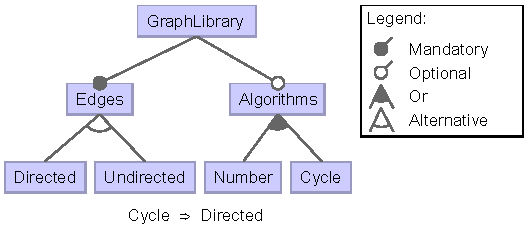
\includegraphics{img/img-fm.pdf}
	\caption{A simple example of a feature model}
	\label{img-fm}
\end{figure}
One of their benefits is the visualization as a feature diagram, providing an overview of the containing features, and their hierarchy and dependencies. In addition, it classifies the features and their dependencies by ordinality (optional/mandatory), logical operator (disjunction/exclusive disjunction) and whether it is abstract or concrete. Furthermore, it contains all information needed to provide a configuration of Features and its validation.

Although feature models can be represented as a propositional expression in CNF, it is typically represented in form of a feature diagram \cite{fmgp}. The feature diagram is structured as a tree. In that manner feature models map the hierarchy of features. The possible relationships of features with a common parent feature are \textit{or}, \textit{alternative} and \textit{and}. In the case of an \textit{or}-group, at least one of the child features has to be selected if the parent feature is selected. Within an \textit{alternative}-group exactly one of the child feature has to be selected if the parent feature is selected. When grouped with an \textit{and}-relation, any number of child features can be selected, if the parent feature is selected. In addition, child features in an \textit{and}-group can be marked as either mandatory or optional.  As features' relations may be of higher complexity than just parent-child relations additional constraints can be noted within a feature model. Constraints can contain any propositional expression.

Figure~\ref{img-fm} shows an example of a simple feature model. The node \textit{GraphLibrary} is the root feature. It's childs are the node \textit{Edges}, that has to be selected due to the mandatory marker, and \textit{Algorithms} that is marked optional. The implemented edge types are \textit{Directed} and \textit{Undirected} from which exactly one has to be chosen as they are mutually exclusive. From the algorithms at least one has to be chosen whenever \textit{Algorithms} is selected. The constraint beneath Figure~\ref{img-fm} implies that if the feature \textit{Cycle} is selected, the edge type needs to be directed.


\subsection{Product configuration}
The variability of a product line is represented by it's feature model, which itself is a set of features with specific interrelations. The process of configuration of a product line describes the steps to derive a product from the product line. To archive this, a user has to select a subset of all the possible features within the product line to meet his requirements \cite{vrt}. However, not all subsets of features result in a valid product. The interrelations of the features restrict the possible combinations of features resulting in a \textit{valid} configuration. If only one of the requirements from the interrelations between the features is validated, no product can be created and the configuration as such is considered \textit{invalid}. For automatic detection of validity, check the next section.

A non-final configuration, that is a configuration that still has some feature choices left to be made, is called a \textit{partial configuration}. A \textit{valid} partial configuration can be useful, as it narrows down the number of possible resulting variations and choices left to make.

During configuration a user selects or deselects features to his needs. This process requires a lot of domain knowledge on the one hand and detailed information about the implementation of each single feature on the other. With growing numbers of features and thus growing numbers of possible products, configuration requires more effort. However, the even greater problem arises from the possible interactions and interrelations of features, which one has to keep track of during configuration \cite{sple-fpt}.

For all the interrelations of features which are contained within the feature model, an automated observation of the resulting constraints supports configuration. It does so by checking for satisfiability after each change in the configuration.


\subsection{Satisfiability} \label{ch:sat}
During creation of the feature model as well as during the configuration of a product, validity must always be taken care of. Validity in this context is described as the satisfiability of the corresponding propositional expression.

The formalism of propositional expressions (see Section~\ref{ch:fm} allows feature models and configurations to be checked for validity. The propositional expression of a (partial) configuration is created on the basis of the propositional expression of the underlying feature model. Each selected feature is appended with a logical \textit{AND} and each specifically unselected feature is also appended with a logical \textit{AND} but gets negated. The resulting expression is then evaluated by a SAT-solver to check for satisfiability \cite{sat-solve}.

Even during configuration this process can be applied to check for invalid partial configurations after each decision. If a partial configuration reduces the valid choices in a single group to a single one, it can be made automatically. This is called \textit{propagation}. The automatic selection or deselection of a features due to propagation of a made selection always results in a valid configuration. Nevertheless the propagated selections can be confusing for the user.